\begin{figure}[htbp]
	\centering
	\includegraphics[width=0.9\textwidth]{./invariants/data/MODEL/n1m_driven/images/3phases/_output_pairplot_reset.png}
	\caption{\textbf{N1M stimulation}:Pairplot of the invariants no reset within cycles. Lower triangle represents the intervals within the same cycle. Upper triangle represents the intervals of one cycle within the next cycle. }
	\label{fig:N1M stimulation pairplot reset}
\end{figure}

\begin{figure}[htbp]
	\centering
	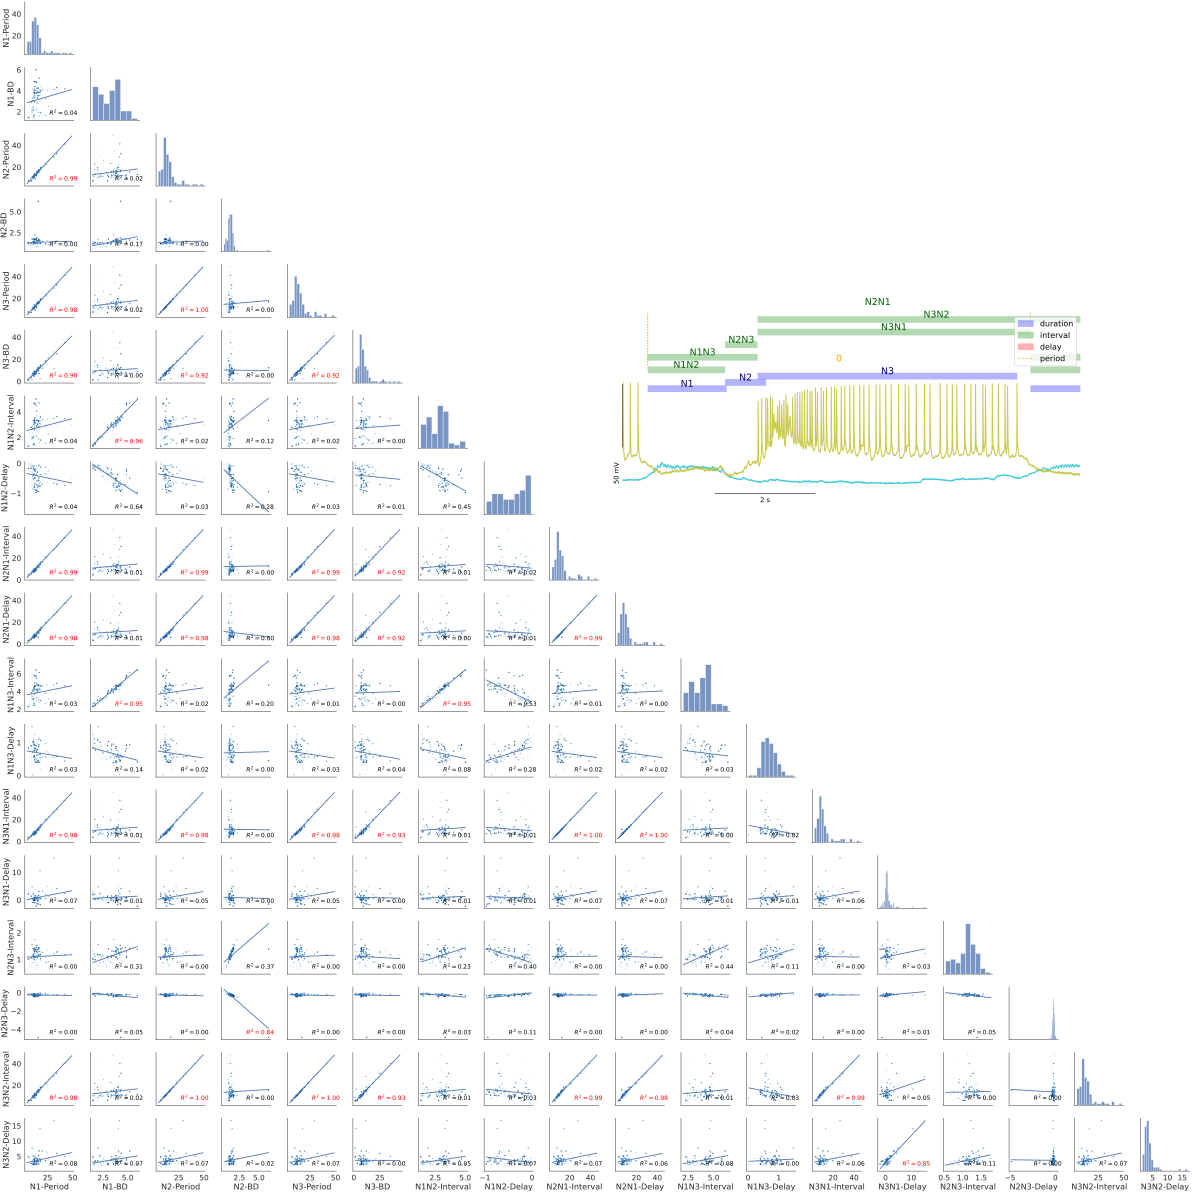
\includegraphics[width=\textwidth]{./img/invariants/data/SUSSEX/prep2/images/3phases/panel_with_pairplot.png}
	\caption{\textbf{Spontaneous case 1}: Panel of intervals distribution and dynamical invariants for the three phases in the CPG for spontaneous activity.}
	\label{fig:prep2 pairplot invariants}
\end{figure}



\begin{figure}[htbp]
	\centering
	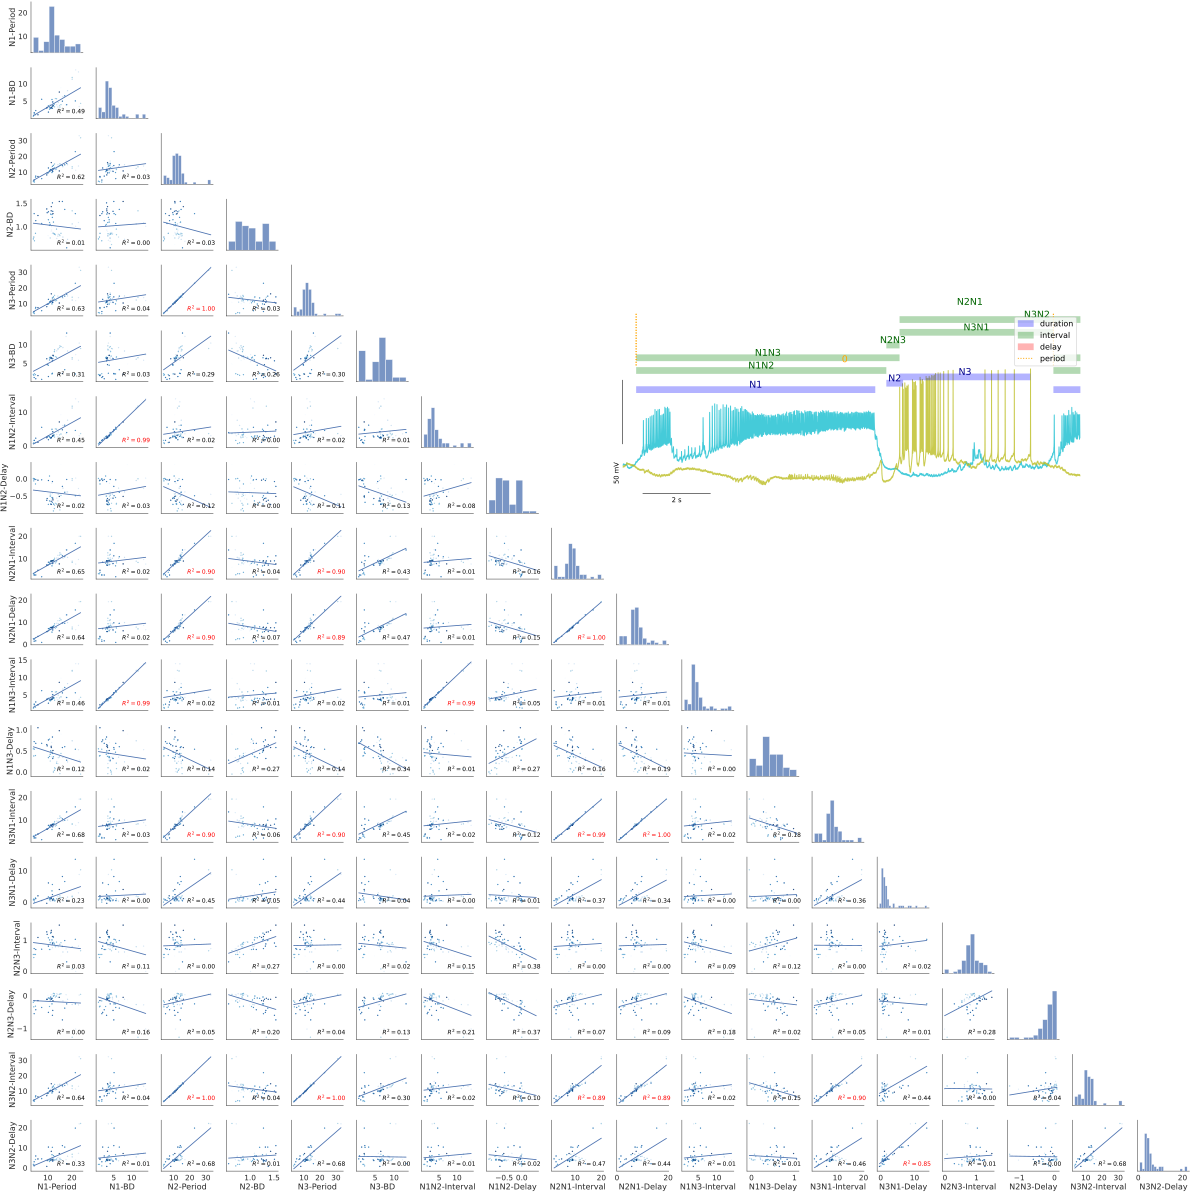
\includegraphics[width=0.9\textwidth]{./img/invariants/data/SUSSEX/prep3/images/3phases/panel_with_pairplot.png}
	\caption{\textbf{Spontaneous case 2}: Panel of intervals distribution and dynamical invariants for the three phases in the CPG for spontaneous activity.}
	\label{fig:prep3 invariants pairplot}
\end{figure}


\begin{figure}[htbp]
	\centering
	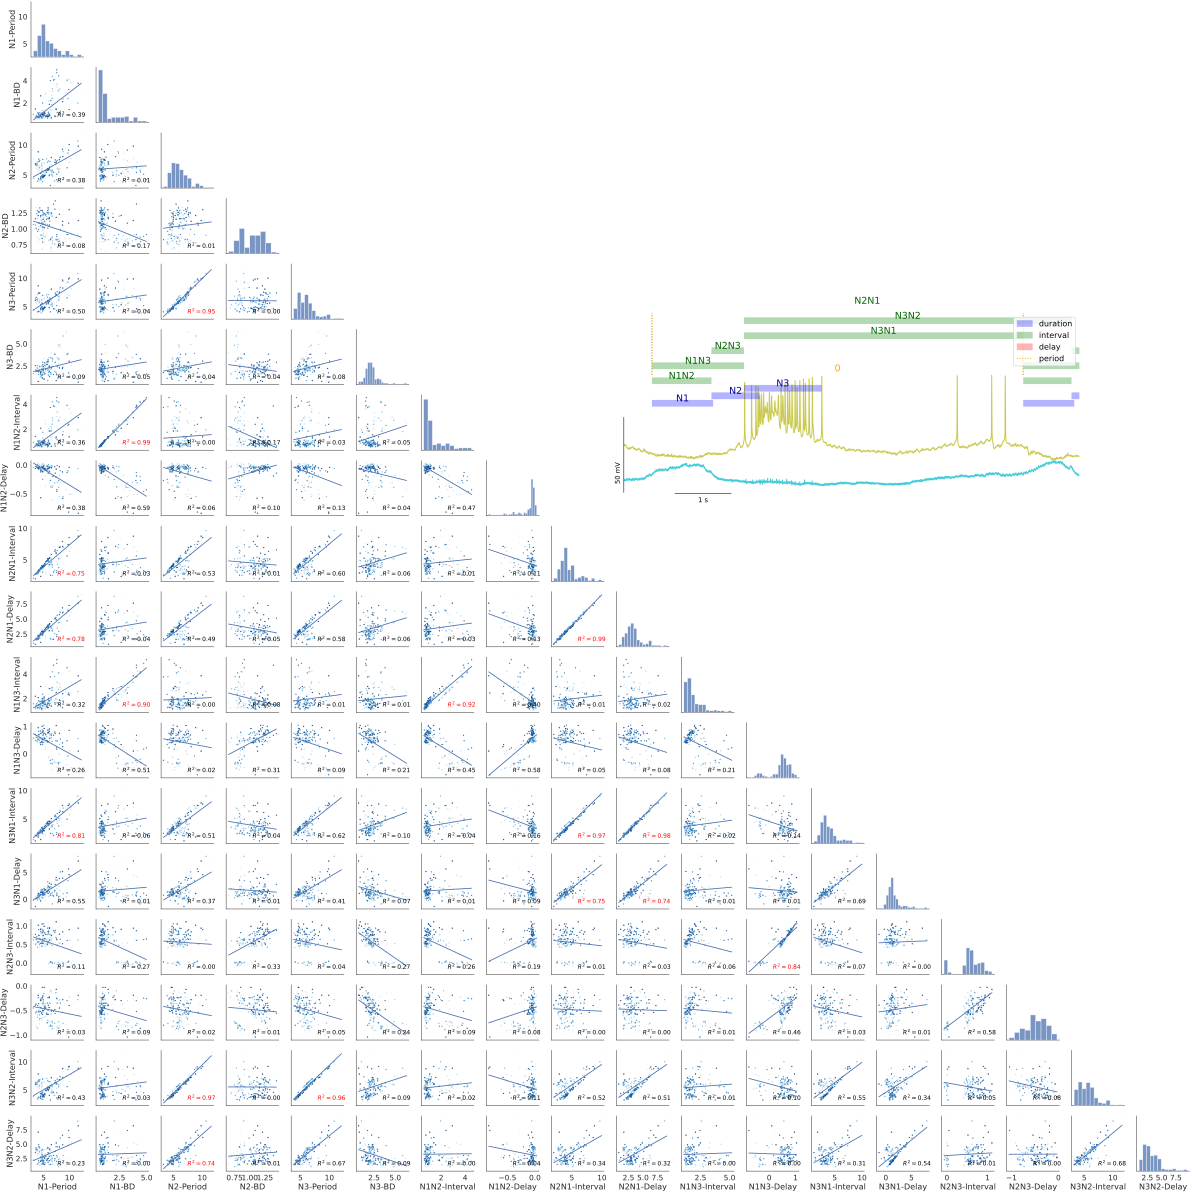
\includegraphics[width=\textwidth]{./img/invariants/data/SUSSEX/prep1/images/3phases/panel_with_pairplot.png}
	\caption{\textbf{Spontaneous case 3}: Panel of intervals distribution and dynamical invariants for the three phases in the CPG for spontaneous activity.}
	\label{fig:prep1 invariants pairplot}
\end{figure}

% sale mal, probablemente pq el fin e inicio de n2v es idéntico
%\begin{figure}[htbp]
%	\centering
%	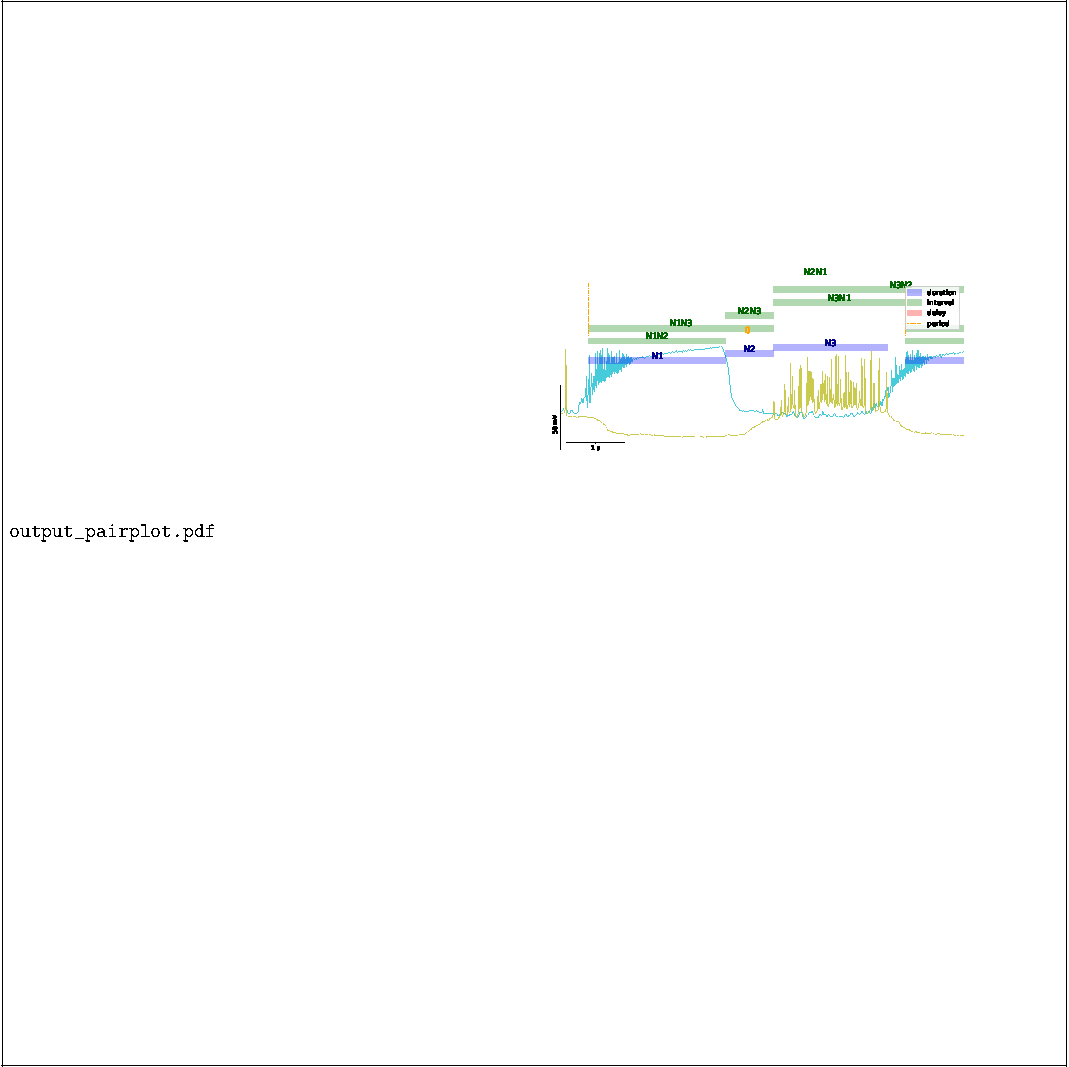
\includegraphics[width=0.9\textwidth]{./img/invariants/data/SUSSEX/CV1a_driven1/images/3phases/panel_with_pairplot.pdf}
%	\caption{\textbf{CV1a driven case1}: Panel of intervals distribution and dynamical invariants for the three phases in the CPG under CV1a stimulation.}
%	\label{fig:cv1a 1 3phases pairplot}
%\end{figure}
%

\begin{figure}[htbp]
	\centering
	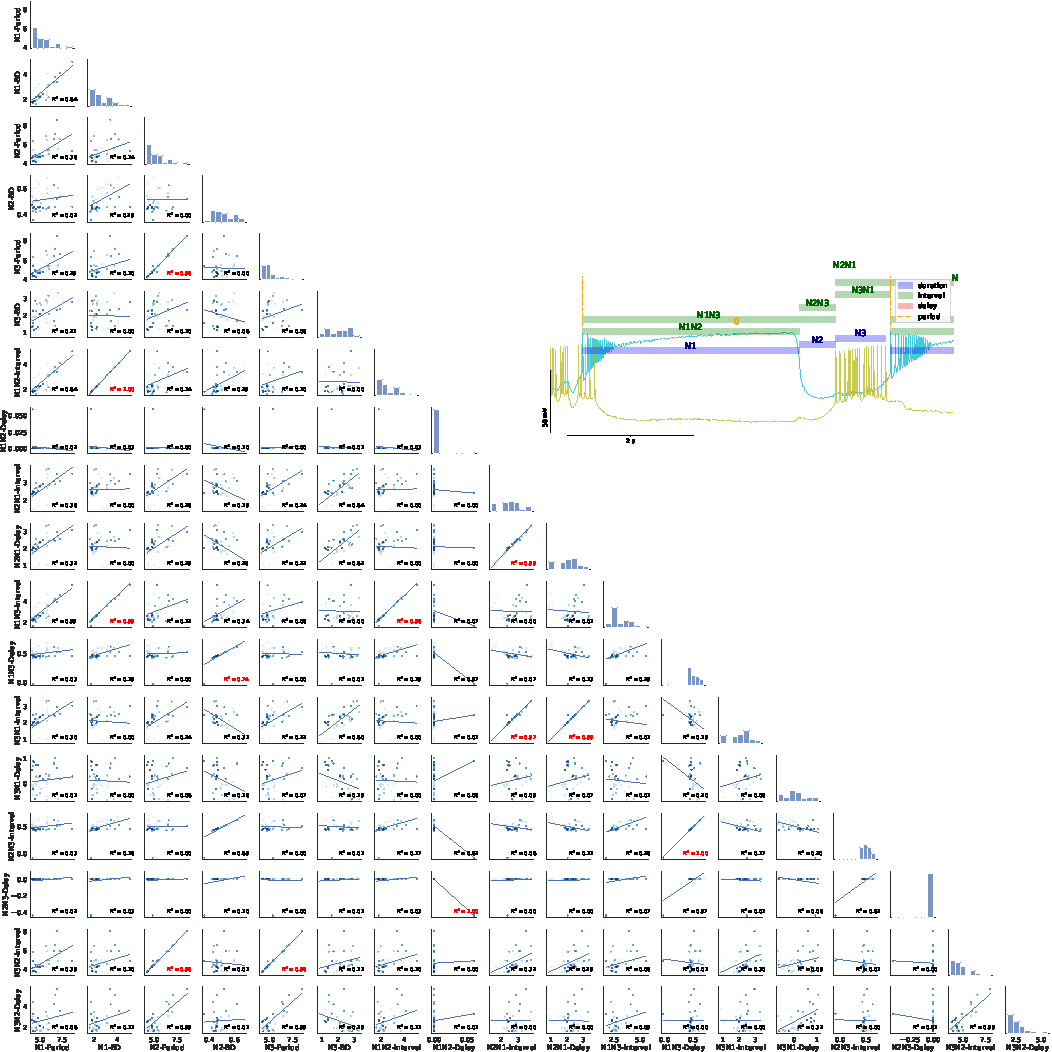
\includegraphics[width=0.9\textwidth]{./img/invariants/data/SUSSEX/CV1a_driven4/images/3phases/panel_with_pairplot.pdf}
	\caption{\textbf{CV1a driven case 4}: Panel of intervals distribution and dynamical invariants for the three phases in the CPG under CV1a stimulation.}
	\label{fig:cv1a 4 3phases pairplot}
\end{figure}



\begin{figure}
	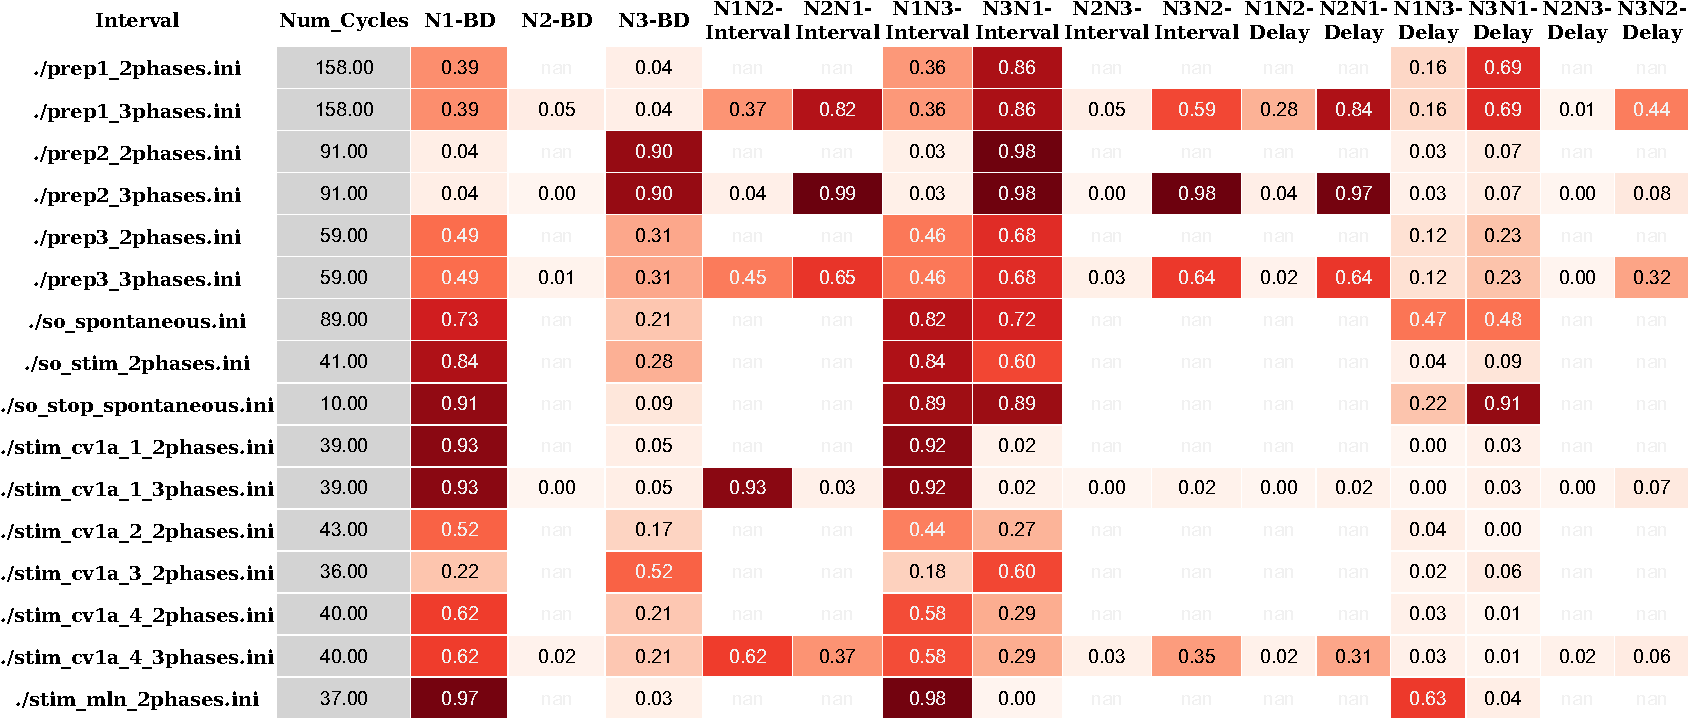
\includegraphics[width=\textwidth]{./img/invariants/styled_table_invariants_r-squared.pdf}
	\caption{Table of $R^2$ values for the linear regression between the period and each interval for all experimental recordings showed in this section.}
	\label{fig:R2 table}
\end{figure}
